% Diagrama 2: Movilidad jerárquica en tres capas
% Compilar con: lualatex movilidad.tex  (sale movilidad.pdf)
\documentclass[tikz,border=16pt]{standalone}
\usetikzlibrary{arrows.meta}
\usepackage{amsmath}
\begin{document}
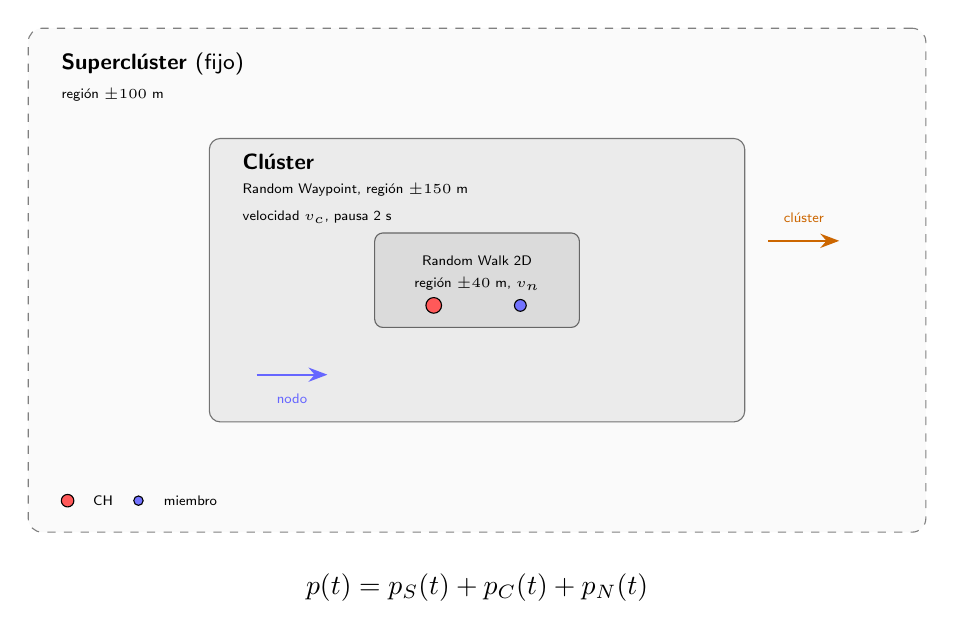
\begin{tikzpicture}[
  font=\sffamily\footnotesize,
  super/.style={draw=black!50, dashed, rounded corners=5pt, fill=black!2},
  cluster/.style={draw=black!55, rounded corners=4pt, fill=black!8},
  nodo/.style={draw=black!60, rounded corners=3pt, fill=black!14},
  ch/.style={circle, draw=black, fill=red!65, inner sep=2pt},
  member/.style={circle, draw=black, fill=blue!55, inner sep=1.5pt},
  arr/.style={-{Stealth[length=2.4mm]}},
]
% Superclúster
\node[super, minimum width=11.4cm, minimum height=6.4cm] (S) at (0,0) {};
\node[anchor=west] at (-5.4,2.75) {\textbf{Superclúster} (fijo)};
\node[anchor=west, font=\sffamily\tiny] at (-5.4,2.35) {región $\pm 100$ m};

% Clúster
\node[cluster, minimum width=6.8cm, minimum height=3.6cm] (C) at (0,0) {};
\node[anchor=west] at (-3.1,1.5) {\textbf{Clúster}};
\node[anchor=west, font=\sffamily\tiny] at (-3.1,1.15)
  {Random Waypoint, región $\pm 150$ m};
\node[anchor=west, font=\sffamily\tiny] at (-3.1,0.8)
  {velocidad $v_c$, pausa 2 s};

% Nodo
\node[nodo, minimum width=2.6cm, minimum height=1.2cm] (N) at (0,0) {};
\node[font=\sffamily\tiny] at (0,0.25) {Random Walk 2D};
\node[font=\sffamily\tiny] at (0,-0.05) {región $\pm 40$ m, $v_n$};

% CH y miembro dentro del nodo
\node[member] at (0.55,-0.32) {};
\node[ch] at (-0.55,-0.32) {};

% Flecha de movimiento del nodo, en el margen izquierdo del clúster
\draw[blue!60, thick, arr] (-2.8,-1.2) -- (-1.9,-1.2);
\node[blue!60, font=\sffamily\tiny] at (-2.35,-1.5) {nodo};

% Flecha de movimiento del clúster, en el margen derecho del superclúster
\draw[orange!80!black, thick, arr] (3.7,0.5) -- (4.6,0.5);
\node[orange!80!black, font=\sffamily\tiny] at (4.15,0.8) {clúster};

% Leyenda de nodos
\node[ch, scale=0.8] at (-5.2,-2.8) {};
\node[anchor=west, font=\sffamily\tiny] at (-5.0,-2.8) {CH};
\node[member, scale=0.8] at (-4.3,-2.8) {};
\node[anchor=west, font=\sffamily\tiny] at (-4.1,-2.8) {miembro};

% Ecuación de composición
\node[font=\sffamily\normalsize] at (0,-3.9)
  {$p(t) = p_S(t) + p_C(t) + p_N(t)$};
\end{tikzpicture}
\end{document}
